\begin{enumerate}[label=\thesection.\arabic*.,ref=\thesection.\theenumi]
\numberwithin{equation}{enumi}

\item Plot the Bode magnitude and phase plots for the following system
\begin{align}
G\brak{s} &= \frac{75\brak{1+0.2s}}{s\brak{s^2+16s+100}}
\label{eq:ee18btech11049_system}
\end{align}
Also compute gain margin and phase margin .
\\
\solution From  \eqref{eq:ee18btech11049_system}, we have 

\begin{align}
G\brak{\j\omega}&=\frac{75\brak{1+0.2\j\omega}}{\j\omega\brak{\brak{\j\omega}^2 + 16\j\omega+100} }
\end{align}
poles = 0 , -8-6j , -8+6j\\
zeros = -5\\
Gain and phase plots are shown in Fig.  \ref{fig:ee18btech11049} 
\begin{figure}[!h]
\centering
  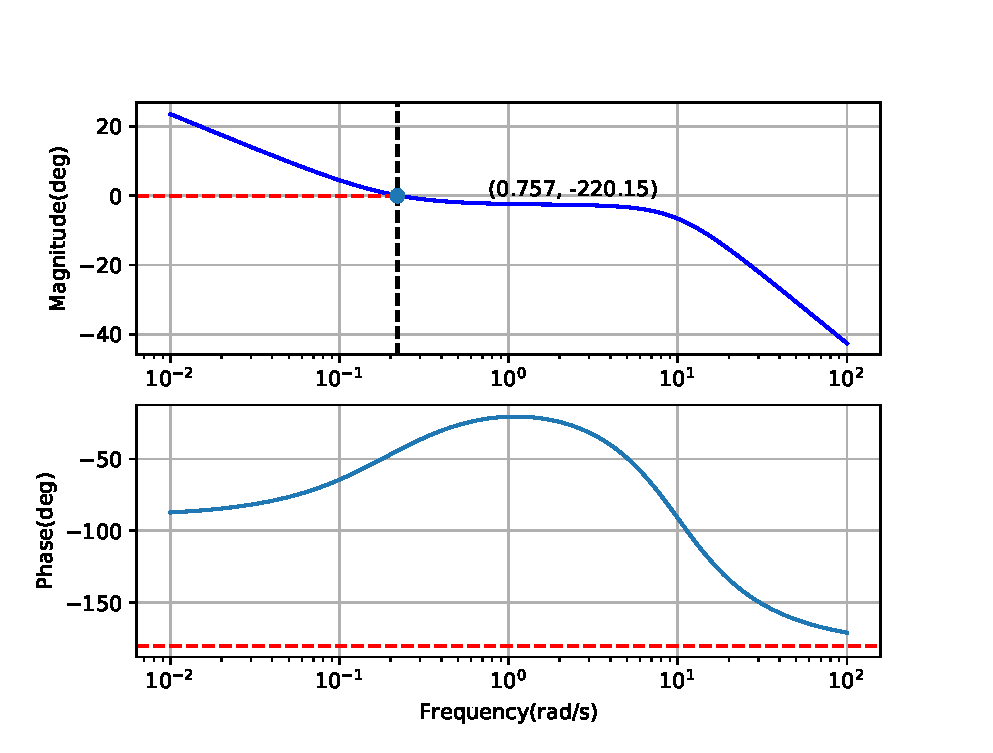
\includegraphics[width=\columnwidth]{./figs/ee18btech11049.eps}
  \caption{a}
  \label{fig:ee18btech11049}
\end{figure}

The following code plots Fig. \ref{fig:ee18btech11049} 

\begin{lstlisting}
codes/ee18btech11049.py
\end{lstlisting}

\item Find $\phase G\brak{\j\omega} + 180\degree$ , where $\omega$ is frequency when gain = 1 . This is known as  {\em phase margin} (PM)
\\
\solution Solving 
\begin{align}
\label{eq:ee18btech11049_gain}
\begin{split}
\abs{G\brak{\j\omega}} &=   \frac{75\sqrt{\omega^2 + 25}}{\omega\sqrt{\brak{\omega+6}^2+64}\sqrt{\brak{\omega-6}^2+64}} 
\\
&= 1,
\end{split}
\end{align}
or from Fig. \ref{fig:ee18btech11049}, the gain crossover frequency 
%
\begin{align}
\implies
\omega_{gc} &=  0.757  \\
\phase{G\brak{\j\omega_{gc}}} &= -88.3 \\
\implies
PM &= 91.7  
% \label{eq:ee18btech11049_phase}
\end{align}

\item Find $-G\brak{\j\omega}  $ db , where $\omega$ is frequency when phase = $-180\degree$ . This is known as  {\em gain margin} (GM)
\\
\solution From Fig. \ref{fig:ee18btech11049} ,we can say that phase  never crosses $-180\degree$ .
So , the gain margin is {\em infinite}.
Which means we can add any gain, and the equivalent closed loop system never becomes unstable.

\end{enumerate}
